\chapter{Verification Setup}\label{sec:Verif}

This section will discuss the security properties used by the Read-Only
section of Verified Boot. 
It will also verify these properties using the Hardware and
Software elements that were outlined in Section 2 and Section 3.
All properties are checked using the C Bounded Model Checker (CBMC).
To check some properties, Hardware modules are converted into C using the ILA toolchain.

\section{Vboot Properties}

The properties that will be verified can be separated into 3 categories: array accesses, program flow, and correctness.
The array access property restricts the writeable addresses in memory to valid array boundaries. 
Program flow properties refer to the program's execution path.
Correctness properties refer to facts about the code such that, if things were
designed successfully, certain states should not be reached.
Together these categories of properties should be enough to prove the security claims made by Vboot.

These properties will be specified in Computation Tree Logic (CTL). 
CTL adds temporal distinctions over propositional logic and this allows one to easily describe how a system changes over time.
The boolean connectives in propositional logic are $\lnot$ for NOT, $\land$ for
AND, $\lor$ for OR, and $p \to q$ for $p$ implies $q$.
CTL describes how propositional logic changes through time.
Table~\ref{ctl_syn} describes the CTL syntax.

\begin{table}[!htbp]
    \centering
    \caption{A description of the CTL syntax}\label{ctl_syn}
    \begin{tabular}{ll}
        \toprule Syntax & Description  \\ \midrule 
        $Xp$ & $p$ is true in the next state\\ 
        $Fp$ & $p$ is true eventually\\ 
        $Gp$ & $p$ is always true\\ \bottomrule
    \end{tabular}
\end{table}

\subsection{Memory Access Locations}\label{my-malloc}

Memory accesses in C are very important because C allows for arbitrary addresses to be accessed. 
Addressing arrays before their starting address or after their final address is known as a buffer overrun and it is one of the most common security vulnerabilities. 
Buffer overruns allow a program to write or read to arbitrary memory. 
In Vboot, a buffer overrun could be used to modify the RSA public keys after they have been read in from secure storage, or it could modify the firmware image after it has been verified as secure. 
Such modifications would defeat the security claims of Vboot and for this reason it is important to prevent the accessing of arrays past the array boundaries.

The equation below describes correct array accesses in CTL. 
\begin{equation}
    G(a \to (i > 0 \land i < size(ptr)))
\end{equation}
In this equation $a$ is any array access, $ptr$ is the start of the array and $i$ is the access offset.
This equation states that for every memory access, the index is greater than 0 so it cannot access memory before the array,  and the index is smaller than the size of the array so memory after the array cannot be accessed.

Array indexing is common enough that CBMC provides checking by default.
However, this check on its own is not strong enough to provide array access security for Vboot. 
This is because Vboot uses pointer manipulation in order to access structures and data within the Image. 
Vboot reads the Image from disk as one contiguous binary. 
After the Image has been loaded, the data structures within the Image use size and offset variables to locate more data.
CBMC is not able to automatically detect if this pointer manipulation results in an access outside of the Image.

The following equation defines correct pointer manipulation in Vboot. 
\begin{equation}
    G(\text{offset}(\text{struct}) + \text{size}(\text{struct}) <
    \text{size}(\text{img}) \land \text{offset}(\text{struct}) > 0)
\end{equation}
In this equation $struct$ is the structure being created from a pointer dereference, and $img$ is the image that it is being pointed to.
The equation states that the offset and size of the struct do not go past the edge of the image and that the offset of the struct does is not negative.
We can assume that the offset is not negative because Vboot offsets should only points forward in the Image.

Together these two properties state that array accesses must be in bounds and that structure dereferencing must be in bounds of the image that is being referenced.
As these are the two memory referencing techniques that have the potential for overrun, these properties protect the system against overrun attacks.

\subsection{Program Flow properties}


There needs to be an ordered constraint on the flow of the program. 
If the program flow is described formally then it will be easy to check that all stages of secure boot were called and in the correct order.
This will catch incorrect programs that skip steps and therefore skip verifying the image, or programs that execute steps out of order and therefore access data that has not been verified yet.
The graph for program flow is shown in Figure~\ref{fig:v_flow}.
When verifying the flow of Vboot it is necessary to note that there are two Images stored in the system, Image A and Image B, and either can be used in the Vboot process. 
It is also necessary to note that Developer mode will skip a step in the verification process, and that this skipped step is a valid part of the Vboot flow.

\begin{figure}[!htbp]
  \centering
  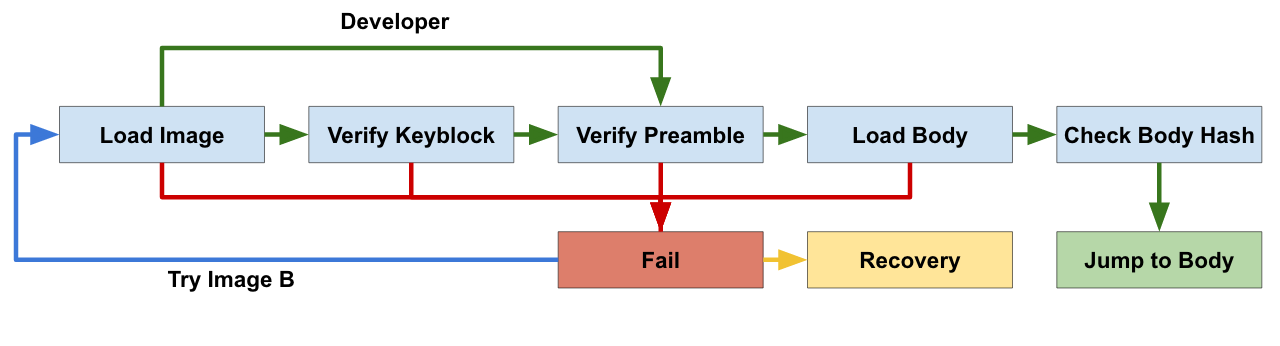
\includegraphics[width=0.8\linewidth]{verification_flow.png}
  \caption[Verified Boot Program Flow]{The logical flow for Vboot.}\label{fig:v_flow}
\end{figure}

Let $s_i$ correspond to the ith stage from Figure~\ref{fig:v_flow} and $s_{ai}$ or $s_{bi}$ correspond to that stage for Image A or Image B respectively.

The equation below states that at any time, we must be in at least one of five stages for either image A or image B.
% Must be in a defined state
\begin{equation}
    G(\bigvee\limits_{i = 0}^{4} s_{ai} \lor s_{bi})
\end{equation}

The equation below states the transitions available for Image A.
Each i\textsuperscript{th} stage can transition either to itself or the following stage.
Image A has the ability to fail and transition immediately to the first stage of attesting Image B.

% Image A transitions to next or to B
\begin{equation}
    G(s_{ai} \to (s_{ai} \lor s_{ai+1} \lor s_{b0}))
\end{equation}

Now we will describe the state transitions for Image B. 
They are similar to Image A but Image B is always tried second and can only transition to the next stage. 
Image B cannot transition back to verifying Image A or it would be possible to have an infinite loop of attesting incorrect images.

% Image B transitions to next
\begin{equation}
    G(s_{bi} \to (s_{bi} \lor s_{bi+1}))
\end{equation}

The final equation refines the transition for state $s_0$ for Image A and B.
In Figure~\ref{fig:v_flow} we can see that state $s_0$ can transition to $s_1$ but it also has a special transition to $s_2$ that is only valid if Developer Mode is enabled.

% State 0 can skip state 1 if in Developer
\begin{equation}
    G(s_0 \to (s_0 \lor s_{1} \lor (M_D \land s_{2})))
\end{equation}

All together these equations fully describe the program flow graph in Figure~\ref{fig:v_flow}. 
If these hold then steps will not be skipped in the verification process and we can be assured that verification of the image will be attempted in order.

\subsection{Correctness properties}

Correctness properties refer to the code itself and help to determine if it has been written correctly.
For Verified Boot, correctness properties focus on the correct attestation of the image and the guarantee that an incorrect Image cannot be marked as correct and loaded for execution.

The following property states that if the system is not in developer mode and the signature verification fails, then the system will eventually reach the failure state for that image.
Here $img$ can refer to either Image A or Image B.
It is important that failure and passing is tracked on an image basis because it is possible for Image A to fail but Image B to pass.

% Signature is correct when not in Dev mode
\begin{equation} \label{eq:sig_cor}
 \lnot M_d \land \lnot \text{verifySignature(img, rootKey)} \to XF (\text{img.pass} = F)
\end{equation}

The following property states that if the hash of the image data does not match the hash stored in the image, then that specific image will eventually fail.

% Hash is correct always 
\begin{equation} \label{eq:hash_cor}
    \text{hash(img.data)} \neq \text{img.hash} \to XF (\text{img.pass} = F)
\end{equation}

The next property checks against the rollback attack. 
Rollback states that all image versions must be greater than or equal to the last seen image version that is kept in secure storage. 
This property claims that if the image version is lower than what is seen in secure storage, then the image will eventually fail.
Rollback is disabled on Recovery Mode and the property below reflects this fact.

% Version should be greater than previously seen when not in recovery
\begin{equation} \label{eq:rollback}
    \lnot M_r \land (\text{img.version} < \text{prevVersion}) \to XF (\text{img.pass} = F)
\end{equation}

The next property checks that if both images fail, then the Vboot process will fail and the system will eventually reboot into recovery mode.

% If both images fail then boot to recovery 
\begin{equation} \label{eq:both-fail}
    \lnot \text{imgA.pass} \land \lnot \text{imgB.pass} \to XF (\text{pass} = F)
\end{equation}

% TODO: maybe add a Dev wipe property

% TODO: maybe add a hardware return correctly property
% TODO: maybe add that if hash(image) = img.hash -> image = img

In the equations above, img refers to the Image to be verified (either Image A or Image B)  and rootKey is Google's public key that has been loaded out of the GBB.
$M_d$ refers to developer mode being active and $M_r$ refers to recovery mode being active.
Img.version is the Image version number and prevVersion is the last seen version that is stored in the TPM\@.

The contrapositive of these properties will be proved.
The contrapositive of a conditional is the inverse of the condition where the antecedent and consequent are negated.
For example, instead of proving that ``if the hash fails then the image will fail'' it will be proved that ``if the image passes then the hash must have passed''. 
This is easier to check and is logically equivalent.


\section{CBMC}

CBMC is a Bounded Model Checking program for the C language that is released by
Carnegie Mellon. 
A Bounded Model Checker is a tool that performs Formal Verification.
Model checking is a way to exhaustively prove whether a given model meets its
specification.
Model checking typically uses propositional logic or temporal logic. 
At its core, CBMC transforms a C program into binary logic and
then uses a SAT solver to check it against the user's specification. 
The specification is user defined, using an API of C functions defined by the
CBMC library. 

% \begin{figure}
%   \centering
%   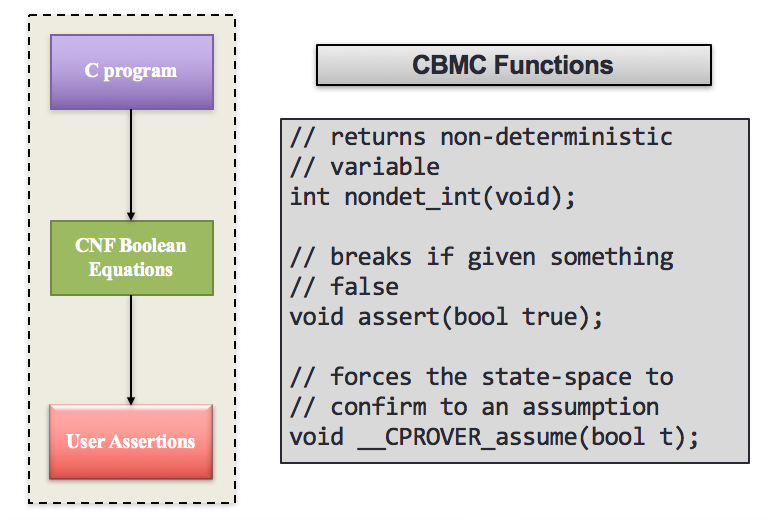
\includegraphics[width=0.7\linewidth]{CBMC_api.png}
%   \caption{The figure on the left describes the transformation that a C
%   program undergoes to be verified. The right describes the CBMC API.}\label{fig:CBMC_api}
% \end{figure}

The CBMC API is very simple.
The list below describes the 3 functions in the CBMC API.

\begin{itemize}
    \item \code{assert(bool e)} -- takes in a boolean expression and throws
        exception if false.
    \item \code{nondet\_int()} -- returns a non-deterministic integer.
    \item \code{assume(bool e)} -- takes in a boolean expression and forces any
        non-deterministic variables to conform.
\end{itemize}

If the \code{assert()} function throws an exception then CBMC will produce a ``counterexample''.
A counterexample lists the program inputs and steps taken that caused the false
assertion.
The \code{nondet\_int()} function is very helpful to model user input to the Vboot process.
Any data that could be modified by the user could feasibly take any
value, and this is represented cleanly by a non-deterministic integer.
CBMC exhaustively checks user assertions against all possible non-deterministic
integer values.

\section{Abstractions}

CBMC was able to be successfully run on portions of the verified boot library and provide information on the satisfiability of various assertions.
Running CBMC on the Read-Only section of Vboot with a full Firmware Image is not possible as the program will consume up to 8GB of RAM on my local machine and then be cancelled.
In order to check properties, abstractions needed to be found such that parts of the Vboot flow could be checked at a single time.

\subsection{Function Over-Abstractions}

The key abstraction used by this thesis is that individual functions are mostly
self contained.
This leads to a natural abstraction at the function definition.
Each Vboot function returns 0 if successful and an error code if it is not successful.
When a function is abstracted away, it is programmed to return a
non-deterministic value.
If the non-deterministic value is zero (success), then the minimal amount of external changes (if any) should be applied to the larger function.
If the abstracted function returns non-zero (error), then the external changes should be replaced with non-deterministic values.

This method is an over-abstraction of a functions found in the Vboot library.
An over-abstraction contains the full set of states found in the original function, plus additional states that would not be possible.
Because the over-abstraction is a super-set of the original states, any properties that are proved with the over-abstraction will also be proved on every state of the original function.
Therefore any properties proved with abstracted functions will also hold if the real functions were left in place.

\subsection{Loop Removal}

Another helpful abstraction is to remove long loops that are present in Verified
Boot.
CMBC performs loop unrolling before it performs any model checking. 
In a program with long loops, the unrolling adds unnecessary complexity and
state to the model and it increases checking time dramatically.
All of Vboots long loops are comparing or copying arrays.
An array compare can be abstracted into a single non-deterministic read on both
arrays.
An array copy can be abstracted into a single non-deterministic write on the
array.
Because the index into the array is non-deterministic in both cases, CBMC will
still perform verification on every acceptable index and find possible
counterexamples.
This abstraction was taken from an earlier thesis that also performed Formal
Verification~\cite{elane}. 

\subsection{Memory Allocation}

The final abstraction is the creation of a simple memory allocation function so
CBMC will handle pointer manipulation correctly.
Vboot data structures contain offsets to other data structures, not full
pointers. 
Vboot uses offsets because the data structures are loaded from disk and there is
no guarantee that the data will be loaded into a specific address.
(There is however, a guarantee that the data will be loaded contiguously)
The following code shows the simple pointer arithmetic needed for offsets.

\begin{equation} \label{eq:ptr}
\begin{split}
    \code{uint32\_t offset = \&data - \&image;} \\
    \code{void *data\_ptr = \&image + offset;} 
\end{split}
\end{equation}

However, CBMC will not perform pointer arithmetic unless the original pointer
was set to a specific value.
A small memory management function was created to assign pointer values to data
structures so CBMC would perform the correct arithmetic.
In this abstraction memory addresses start at 0x0 and increase as needed.
Memory is never reclaimed.
The idea for this abstraction originated from the work done in modeling memory
by Franjo Ivancic\cite{eff-model-check}.

\subsection{Google's Assertions}

Google has already created a Unit Test Framework for the Verified Boot process.
This framework tests various properties of each function.
The testing framework also relied on propositional logic and assert statements.
With minor changes to the framework the each test could also be verified using Formal Verification tools.

The verification work done in this paper is still strictly better than the existing tests. 
The existing assertions are now proven formally on any input, and more advanced properties were able to be proven. 
Google's framework also stubs out any calls to hardware, meaning that it 
will not catch any errors across the Hardware Software boundary.

\chapter{Verification Results}\label{sec:VerifResults}

 \begin{figure}[!htbp]
   \centering
   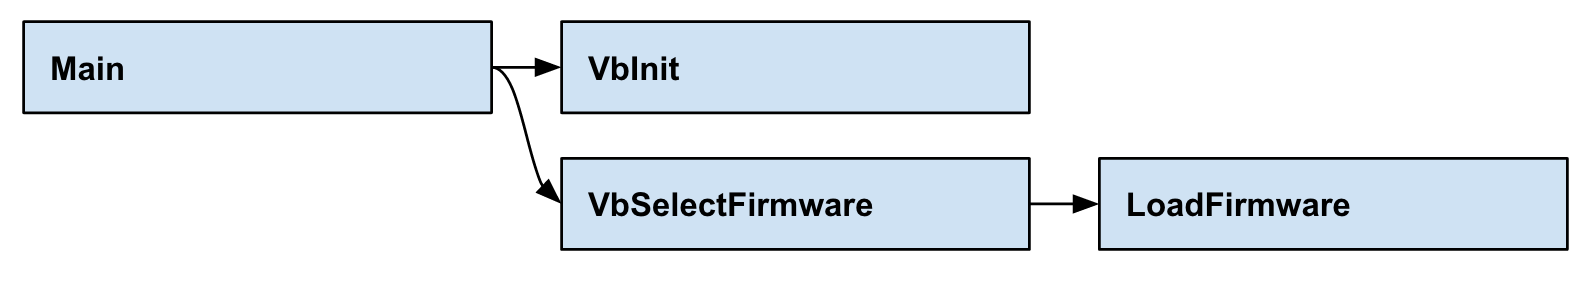
\includegraphics[width=0.8\linewidth]{gen_flow.png}
   \caption[Vboot General Call Graph]{The general call graph of functions for Vboot. A full overview is available in the Appendix.}\label{fig:allflow}
 \end{figure}

This section describes the verification tests on Vboot using CBMC\@.
Each subsection begins with a diagram showing the functional call graph of the section of code is being verified.
The diagrams are color-coordinated as followed.
The blue functions are fully software functions that are implemented in the Vboot Library.
The purple functions connect to the SHA accelerator on a real platform, 
but use a software abstraction for verification.
The red functions connect to the TPM on a real platform, and are 
verified on either the TPM ILA or the TPM C abstraction.

The following sections focus on verification at the function level.
The sections are organized so the larger functions are in the beginning and the smaller, more specific functions are at the end. 
The function being verified in a specific section is left unmodified, but some of the connecting functions are replaced with abstractions.
These abstractions all follow the idea of an ``over-abstracted'' function discussed in the last section.
These abstractions are acceptable because the real functions are also verified in later sections.
The abstracted functions can be seen in the code repo\cite{my-repo}.

At the end of each section there will be a table describing the results of each CBMC run.
CMBC uses an implementation of a SAT solver known as the MiniSat solver\cite{minisat}.
This solver outputs unSAT if the assertions hold and SAT if they do not. 
The ``steps'' column is the number of C lines that were stepped through to reach the proof conclusion.
The ``VCC'' column is the number of user assertions that were being verified.
The ``time'' column is the total clock time that the verification ran for.
The ``memory'' column is the maximum memory usage in Megabytes.

All results were gathered on Princeton's SAT8 server. 
The SAT8 server contains an Intel Xeon E5645 CPU and has 128 Gigabytes of RAM.

\section{VbSelectFirmware}

\begin{figure}[!htbp]
  \centering
  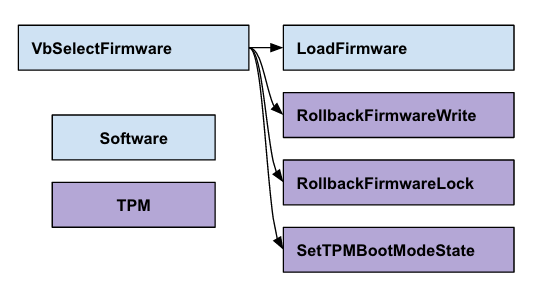
\includegraphics[width=0.5\linewidth]{vb_sel_fw.png}
  \caption[VbSelectFirmware Call Graph]{The call graph of functions for VbSelectFirmware}\label{fig:vbselfw}
\end{figure}

The VbSelectFirmware function mostly acts as a wrapper to LoadFirmware.
It is responsible for loading data and accessing the TPM\@.
VbSelectFirmware is responsible for loading a chosen Image's version number into the TPM and locking the TPM's data. 
This functionality is what prevents rollback attacks across multiple boots.
VbSelectFirmware is also responsible for loading the TPM's PCR0 with a hash of the system's boot flags.
This functionality prevents the system from changing boot flags mid-boot without detection.  

Here are the tests run on VbSelectFirmware:
\begin{itemize}
 \item  TPM locking -- tests that it is not possible for VbSelectFirmware to return success if it is unable to lock the TPM
 \item  LoadFirmware -- tests that it is not possible for control to pass to an Image if it is not selected by LoadFirmware
 \item  Array accesses -- check for all possibilities of array bounds errors.
\end{itemize}

\begin{table}[!htbp]
    \centering
    \caption{CBMC tests on VbSelectFirmware function}\label{sfw_results}
    \begin{tabular}{lrrrrr}
        \toprule
        test name & steps & VCCs & time (s) & memory (Mb) & sat/unsat  \\ \midrule
        TPM locking & 5269 & 6 & 2.42 & 164 & unsat \\
        LoadFirmware & 5264 & 2 & 2.64 & 164 & unsat \\
        Array Accesses & 5257 & 10 & 2.67 & 165 &  unsat \\\bottomrule
    \end{tabular}
\end{table}

The CBMC tests run successfully and in a short time.
The VbSelectFirmware function does little work on its own, so there is not much to verify.
As we will see in the next section, most of the work is done in LoadFirmware. 

\section{LoadFirmware}

\begin{figure}[!htbp]
  \centering
  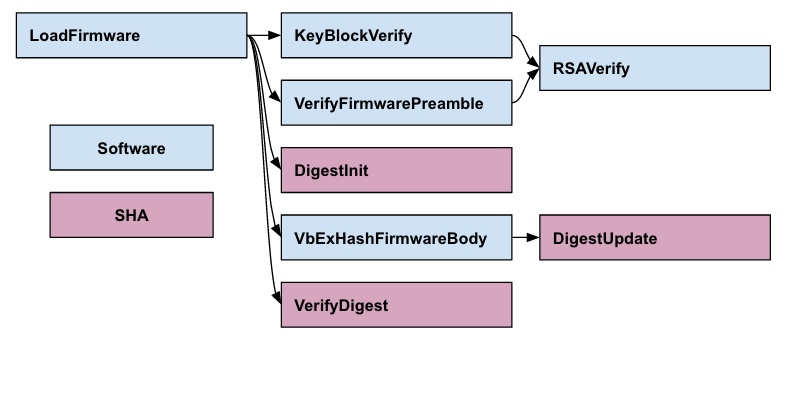
\includegraphics[width=0.7\linewidth]{loadfw.png}
  \caption[LoadFirmware Call Graph]{The call graph of functions for LoadFirmware}\label{fig:loadfw}
\end{figure}

LoadFirmware drives most of Vboot's Image attestation process.
LoadFirmware is responsible for attesting the Keyblock, Preamble, and Image.
When LoadFirmware returns, it will have set the pass or fail statuses of both Images, and control will pass to a working Image.

The CBMC test results for this function can be seen in Table~\ref{ldfw_results}. 
Below is an itemized list of what each test is verifying.

\begin{itemize}
 \item  Google Assertions -- this test replaces Google's assertions with CBMC assertions and checks that none of them are violated under any inputs
 \item  Rollback test -- tests that under no input conditions will LoadFirmware choose an Image with a lower version number (see Property~\ref{eq:rollback}).
 \item  Rollback/rec  -- this test is supposed to find a counter-example. It tests for rollback conditions without realizing that rollback is allowed under recovery. 
 \item  Hash Failure -- tests that it is impossible to verify an image as correct if hashing the Image Body returns an error (see Property~\ref{eq:hash_cor}).
 \item  RSA Failure -- tests that is impossible to verify an image as correct if verifying either the Keyblock or Preamble returns an error (see Property~\ref{eq:sig_cor}).
 \item  Array accesses -- check for all possibilities of array bounds errors.
\end{itemize}

\begin{table}[!htbp]
    \centering
    \caption{Verifying LoadFirmware function}\label{ldfw_results}
    \begin{tabular}{lrrrrr}
        \toprule
        test name & steps & VCCs  & time (s) & memory (Mb) & sat/unsat  \\ \midrule
        Google Assertions & 6460 & 34 & 123 & 2312 & sat \\
        Rollback     & 4125 & 1 & 4.27 & 259 & unsat \\
        Rollback/rec & 4123 & 1 & 4.68 & 394 & sat \\
        Hash Failure & 4182 & 2 & 4.45 & 258 & unsat \\
        RSA  Failure & 4180 & 2 & 4.45 & 258 & unsat \\
        Array Accesses & 4130 & 57 & 126 & 2487 & unsat \\\bottomrule
    \end{tabular}
\end{table}

\begin{table}[!htbp]
    \centering
    \caption{Verifying LoadFirmware function (with memory addressing)}\label{ldfw_results_malloc}
    \begin{tabular}{lrrrrr}
        \toprule
        test name & steps & VCCs  & time (s) & memory (Mb) & sat/unsat  \\ \midrule
        Google Assertions & 6460 & 34 & 3799 & 60496 & unsat \\
        Rollback, Hash, RSA & 2858 & 6 & 3733 & 59874 & unsat \\\bottomrule
    \end{tabular}
\end{table}

We can see from these tests that CBMC is working as expected.
The counter example of the ``rollback/rec'' test quickly pointed the user to the counterexample where the Recovery Mode allowed rollback.
All of the assertions were checked in a short time without the memory allocating technique outlined in Section~\ref{my-malloc}. 
However, CBMC was able to find counterexamples to the Google Assertions because array addressing was not working correctly.
The counterexamples involved Preamble and Keyblock addresses that were outside the bounds of the original Image.
These addresses allowed Vboot to behave insecurely because the array addressing was not working correctly.
However, we can see that Vboot checks for this when the memory addressing technique is applied in Table~\ref{ldfw_results_malloc}

Table~\ref{ldfw_results_malloc} shows the same tests with the memory allocating technique implemented.
We can see that CBMC takes much longer to proof the assertions, but the Google Assertions are working correctly.
Without the memory allocation technique, it would be reasonable to assume that a generic personal computer could run Formal Verification with CBMC. 
The first tests finished in under two minutes and the most memory used was roughly 2 Gb of RAM.
However, with CBMC, the tests take up to an hour and use up to 60 Gb of RAM.
It is extremely unlikely that a personal computer would have 60 Gb of RAM, meaning that CBMC can only be run on a large server for this type of verification. 

\section{TPM TLCL functions}

\begin{figure}[!htbp]
  \centering
  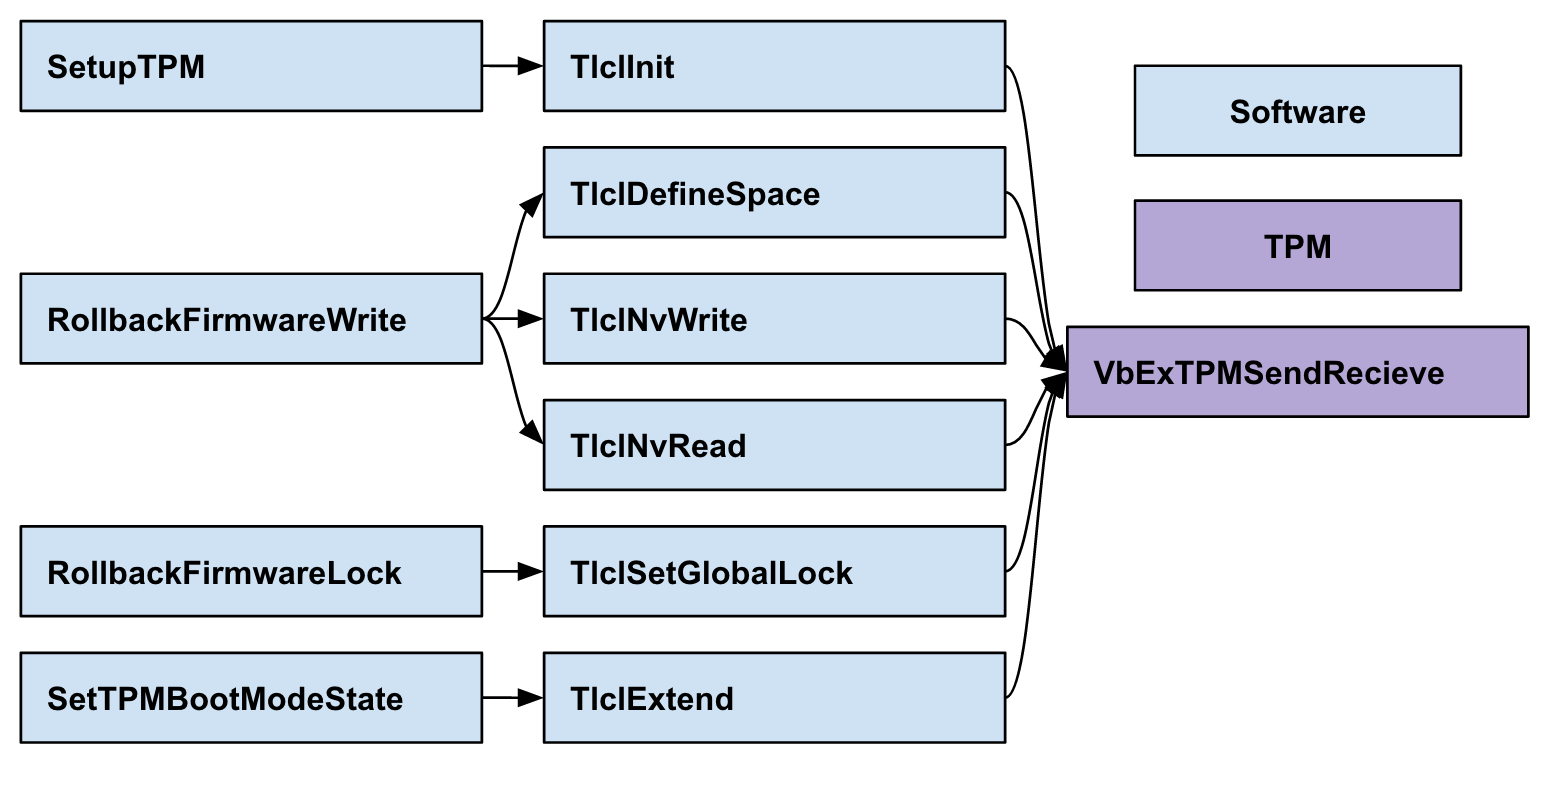
\includegraphics[width=0.6\linewidth]{tpm_fun.png}
  \caption[TPM Call Graph]{This shows the Vboot call graph for the TPM functionality}\label{fig:tpm_call_graph}
\end{figure}

The TPM Lightweight Command Library (TLCL) is Google's library for building and sending TPM commands.
Each function corresponds to a single TPM command and a single call to the TPMSendReceive function.
These tests verify correct functionality for the TLCL commands that are used by Vboot. 

\begin{itemize}
   \item Error Handling --  the TPM returns success only if the TPM command completes successfully
    \item SetupTPM -- the TPM is initialized successfully with well-defined states
    \item  RollbackFirmwareWrite -- the RollbackFirmwareWrite function sends the write value to the TPM unmodified and no TPM assertions are broken
    \item  RollbackFirmwareLock -- the RollbackFirmwareLock function will always lock the correct section and no TPM assertions are broken
    \item SetTPMBootModeState -- the SetTPMBootModeState function sends the PCR value to the TPM unmodified and no TPM assertions are broken

\end{itemize}

\begin{table}[!htbp]
    \centering
    \caption{CBMC tests on TLCL Library}\label{TLCL_results}
    \begin{tabular}{lrrrrr}
        \toprule
        test name & steps & VCCs & time (s) & memory (Mb)& sat/unsat  \\ \midrule
        Error Handling & 34639 & 10 & 11 & 1579 & unsat \\
        SetupTPM & 613418 & 140 & 1674 & 6960 & unsat \\
        RollbackFirmwareWrite & 478639 & 108 & 952 & 5447 & unsat \\
        RollbackFirmwareLock & 17450 & 4 & 7 & 369 & unsat \\
        SetTPMBootModeState & 34621 & 8 & 11 & 397 & unsat \\ \bottomrule
    \end{tabular}
\end{table}

The longest test run in this section finishes in thirty minutes and uses 6.7 Gb of RAM.
It is likely that these tests could be run on a high-end laptop.
All tests completed successfully. 
In addition to the individual test assertions, the tests also include the TPM assertions outlined in the next section.

\section{TPM Send and Receive}

Each TLCL function passes through the single function TpmSendReceive.
TpmSendReceive sends data to and from the TPM with the TPM command registers outlined in Section~\ref{tpm_cmd_regs}. 
The TpmSendReceive function must be verified against all possible inputs to ensure that the TPM cannot be put into an unwanted state.
The assertions outlined in this section are also verified against the TLCL library functions in the previous section.
While the previous section verified TPM correctness during well-defined commands, this section verifies the TPM against sending and receiving random data.

\begin{itemize}
   \item Liveness -- Checks that TpmSendReceive will not enter a state where it polls on an unchanging TPM register
   \item Data Send -- Checks that TpmSendReceive will only return success if the TPM has read each sent byte successfully
   \item Data Receive -- Checks that TpmSendReceive will not return if the TPM still has data to send 
\end{itemize}

\begin{table}[!htbp]
    \centering
    \caption{CBMC tests on VbExTpmSendReceive function}\label{tpmSR_results}
    \begin{tabular}{lrrrrr}
        \toprule
        test name & steps & VCCs & time (s) & memory (Mb) & sat/unsat  \\ \midrule
        Liveness & 20369 & 2217 & 359 & 56434 & unsat \\
        Data Send & 21703 & 259 & 34 & 3991 & unsat \\
        Data Receive & 20231 & 2 & 391 & 61040 & unsat \\ \bottomrule

    \end{tabular}
\end{table}

Again, everything is able to verified successfully. 
The longest command finished in 6 minutes and used 15 Gb of RAM. 
These commands would likely have to be run on a high-end Desktop or Server because of their high RAM usage.

The Liveness property was verified in a unique way compared to other properties in this report.
The Liveness property ensures that the TPM firmware will not be stuck in an infinite loop.
An infinite loop will result if the firmware polls a TPM register that will never change, or if the TPM returns an infinite amount of data.
These situations are checked against using CBMC's loop unrolling.
Each \code{while} loop is unrolled a pre-defined number of times.
CBMC inserts assertions that the loops will not be accessed more than their unroll limit.
Because the loop unrolling assertions hold for every possible input, we can be sure that each loop is run a finite number of times.
